\chapter{Diseño de un algoritmo corrección atmosférica de aguas turbias para sensores con bandas en el SWIR lejano}
\label{pca}

Como ya hemos visto en capítulos anteriores, en aguas ópticamente complejas como las del RdP, el habitual supuesto de agua negra en las bandas del NIR se torna usualmente inválido debido a la alta retrodispersión causada por la alta concentración de material particulado en suspensión presente en el agua (\S \ref{int:s:ACblackPixelNIR}). A su vez, hemos descrito que los esquemas iterativos basados en las bandas del NIR tampoco suelen brindar buenos resultados en imágenes MODIS debido a la saturación de dichas bandas, o bien debido a falencias en el modelo bioóptico utilizado para estimar la reflectancia del agua en el NIR y/o el VIS (\S \ref{int:s:ACiterNIR}). Si bien la estrategia basada en el supuesto de agua negra en las bandas del SWIR ya fue planteada anteriormente (\S \ref{int:s:ACswir}), en este capítulo exploraremos la posibilidad de utilizar esta misma estrategia pero con un esquema extrapolativo diferente, basado en la descomposición por Análisis de Componentes Principales (\textit{Principal Component Analysis}, PCA) de un conjunto de simulaciones de reflectancias a TOA en las que sólo se consideran la atmósfera y el efecto de la interfase (es decir, $\rho_{w}=0$). La diferencia esencial es que en el esquema de extrapolación por PCA las magnitudes utilizadas para la extrapolación se obtienen a partir de la matriz de covarianza de las simulaciones y no de parámetros prefijados como la amplitud de la señal y el cociente de las bandas correctoras, $\epsilon(\lambda_{1},\lambda_{2})$. A su vez, si bien el enfoque original de este esquema implica la estimación de la reflectancia del agua en la banda del NIR centrada en 865 nm, analizaremos la plausibilidad en la estimación directa de otras relfectancias del agua a partir de este método para determinar hasta qué banda es posible una extrapolación directa desde el SWIR. Para estimar estas componentes en la señal de tope de atmósfera (TOA), el peso de cada uno de los autovectores de la matriz de covarianza del conjunto de simulaciones es determinado a partir de las bandas en el SWIR para cada píxel. El algoritmo fue testeado teóricamente a partir de un conjunto de simulaciones a TOA en que fueron introducidas condiciones atmosféricas y mediciones in-situ de reflectancias marinas del RdP. Diversos esquemas fueron analizados utilizando distintas combinaciones de bandas \textit{correctoras} en el SWIR presentes en los sensores MODIS (Aqua y Terra), Suomi-NPP/VIIRS, Sentinel-2/MSI y SABIA-Mar/VNIR-SWIR.

% Estos conjuntos se diferencian entre sí por su correlación con el NIR y la validez del píxel negro. Sin considerar el ruido del sensor, el esquema con mejor desempeño corresponde a aquel donde la señal marina es despreciable para las bandas SWIR consideradas: 1640 nm (SABIA-Mar/MODIS) y 2130 nm (MODIS).



\section{Introducción}
\label{pca:s:introduccion}

Si bien existen esquemas de CA basados e

La corrección atmosférica estándar clásica aplicada a imágenes Sea-WIFS (Sea Wide Field-of-View Sensor) y MODIS (Moderate Resolution Imaging Spectroradiometer) utiliza dos bandas en el infrarrojo cercano (NIR) a 765 y 865 nm, suponiendo una contribución nula de radiación proveniente del agua (píxel negro) en estas bandas [1]. El proceso consiste en i) estimar la componente atmosférica a partir de estas bandas (aprovechando la ausencia de la señal marina), y ii) extrapolar la señal a las bandas visibles (VIS) (las que poseen información útil). Para los casos en que existe alguna señal marina leve en el NIR, se ejecuta un proceso iterativo para estimar esta componente para luego restarla de la señal total y así recuperar la condición de píxel negro, y proceder como de costumbre hacia la extrapolación al VIS [2]. En aguas con concentraciones elevadas de partículas suspendidas (SPM), que retrodispersan fuertemente en el NIR, la señal a 765 y 865 nm ya no es moderada e incluso excede a veces los valores de saturación del sensor. En estos casos, este procedimiento iterativo ya no es operativo y se necesitan otras alternativas.

Muchos autores han propuesto utilizar las bandas de onda corta infrarroja (SWIR) como alternativa (por ejemplo, 1240, 1640 y 2130 nm en MODIS) [3] - [5]. En esta región espectral, la absorción de agua aumenta drásticamente, lo que hace que la suposición de píxeles negros se mantenga a pesar de la presencia de concentraciones altas de sedimentos fuertemente retrodispersivos. Aun así, se ha encontrado que en la región de turbidez máxima en el RdP, la reflectancia a la banda MODIS de 1240 nm todavía no es despreciable [6], lo que socava el rendimiento del algoritmo estándar NIR-SWIR desarrollado por Shi-Wang 2007 [3] y Wang-Shi 2007 [4] en esta región. Como alternativa, se ha propuesto utilizar regiones auxiliares de agua clara en las imágenes donde se asume la suposición de píxeles negros y utilizar la información de aerosol recuperada de estos píxeles en toda la imagen [7].


En el presente capítulo, se presenta y testea teóricamente un esquema de corrección atmosférica preliminar para estimar la reflectancia marina en la banda NIR a 865 nm para que se pueda restar de la señal total para recuperar la condición de píxel negro. Básicamente consiste en descomponer la señal atmosférica en componentes principales (PCA) y estimar sus pesos correspondientes utilizando la reflectancia en las bandas SWIR en cada píxel. Las bandas SWIR que se probaron corresponden a MODIS (Aqua y Terra), Visible Infrared Imaging Radiometer Suite (Suomi-NPP/VIIRS) y Sentinel-2/MSI. Es importante recalcar que, si bien inicialmente el esquema de corrección atmosférica desarrollado en este trabajo estuvo enfocado en las bandas del Satélite Argentino Brasileño para Información del Mar (SABIA-Mar), el esquema no es actualmente alicable a dicho sistema. Esto se debe a que la banda de %%% TODO.
Una ventaja de este procedimiento es que no se basa ni en regiones auxiliares de agua clara en las imágenes (como en Dogliotti et al. 2011 [7]) ni en árboles de decisión para definir aguas turbias y no turbias (como en el NIR- Enfoque SWIR [4]) que producen dificultades en las zonas de transición.


\begin{table}[htb]
\tiny
\caption{Bandas de los sensores en que el algoritmo SOS-PCA fue testeado teóricamente. En verde se marcan las bandas en las que la hipótesis de píxel negro (agua negra) es estrictamente válida. En amarillo, las bandas en que dicha hipótesis se vulnera únicamente a concentraciones de sedimentos muy elevadas (e.g. frente de turbidez del RdP). En rojo, bandas inutilizables para nuestros propósitos debido a fuerte absorción de componentes atmosféricos ($O_{2}$, $H_{2}O$).}
\begin{tabular}{|l|l|l|l|l|}
\hline
\textbf{Aqua/MODIS}         & \textbf{Terra/MODIS}        & \textbf{Suomi-NPP/VIIRS}    & \textbf{Sentinel-2/MSI}     & \textbf{SABIA-Mar/VNIR-SWIR}\\ \hline
                            &                             &                             &                             & 380                         \\ \hline
412                         & 412                         & 410                         &                             & 412                         \\ \hline
443                         & 443                         & 443                         & 443                         & 443                         \\ \hline
469                         & 469                         &                             &                             &                             \\ \hline
488                         & 488                         & 486                         & 490                         & 490                         \\ \hline
                            &                             &                             &                             & 510                         \\ \hline
531                         & 531                         &                             &                             & 531                         \\ \hline
551                         & 551                         & 551                         &                             & 555                         \\ \hline
555                         & 555                         &                             & 560                         &                             \\ \hline
                            &                             &                             &                             & 620                         \\ \hline
645                         & 645                         &                             &                             &                             \\ \hline
667                         & 667                         &                             & 665                         & 665                         \\ \hline
678                         & 678                         & 671                         &                             & 680                         \\ \hline
                            &                             &                             & 705                         & 710                         \\ \hline
748                         & 748                         & 745                         & 740                         & 750                         \\ \hline
                            &                             &                             &                             & 765                         \\ \hline
                            &                             &                             & 783                         &                             \\ \hline
                            &                             &                             & 842                         &                             \\ \hline
859                         & 859                         &                             &                             &                             \\ \hline
869                         & 869                         & 862                         & 865                         & 865                         \\ \hline
                            &                             &                             & {\color[HTML]{FE0000} 945}  &                             \\ \hline
                            &                             &                             &                             & 1044                        \\ \hline
{\color[HTML]{FFCB2F} 1240} & {\color[HTML]{FFCB2F} 1240} & {\color[HTML]{FFCB2F} 1238} &                             & {\color[HTML]{FFCB2F} 1240} \\ \hline
                            &                             &                             & {\color[HTML]{FE0000} 1375} &                             \\ \hline
{\color[HTML]{34FF34} 1640} & {\color[HTML]{34FF34} 1640} & {\color[HTML]{34FF34} 1601} & {\color[HTML]{34FF34} 1610} & {\color[HTML]{34FF34} 1640} \\ \hline
{\color[HTML]{34FF34} 2130} & {\color[HTML]{34FF34} 2130} & {\color[HTML]{34FF34} 2257} & {\color[HTML]{34FF34} 2190} &                             \\ \hline
\end{tabular}
\end{table}

\section{Descripción del algoritmo}

Para simular las reflectancias a TOA para los sensores SABIA-Mar y MODIS, se ejecutó el código de transferencia radiativa CNES-SOS v5.0 (SOS: Sucesivos órdenes de dispersión) [8] utilizando un conjunto de valores de entrada especificados por datos de campo recopilados en la región RdP y por valores estándar encontrados en la literatura.
El rango espectral cubierto abarca todas las bandas MODIS, VIIRS, MSI en la región VIS-NIR-SWIR (Tabla I). En esta tabla, las bandas donde la reflectancia marina no es despreciable en aguas turbias y necesita estimarse se indica en naranja y las bandas SWIR (que se supone son negras) utilizadas para la corrección atmosférica se muestran en rojo. Las reflectancias para cada banda se calcularon utilizando las funciones de respuesta espectral (SRF) correspondientes informadas por la NASA [9] en el caso de MODIS, y utilizando SRF de forma cuadrada definidos por los centros y anchos de banda en el caso del sensor SABIA-Mar.



Para tener en cuenta el efecto de dispersión de Rayleigh producido por las moléculas de aire, se obtuvieron los valores de espesor óptico de Rayleigh y factor de depolarización molecular computados por Bodhaine et al. 1999 [10]. Los escenarios atmosféricos de aerosoles utilizados corresponden a combinaciones previsibles de los escenarios estándar propuestos por la Organización Meteorológica Mundial (WMO) [11] (continental, marítimo, urbano) para la región del Río de la Plara(ver Tabla II).

\begin{figure}
\centering
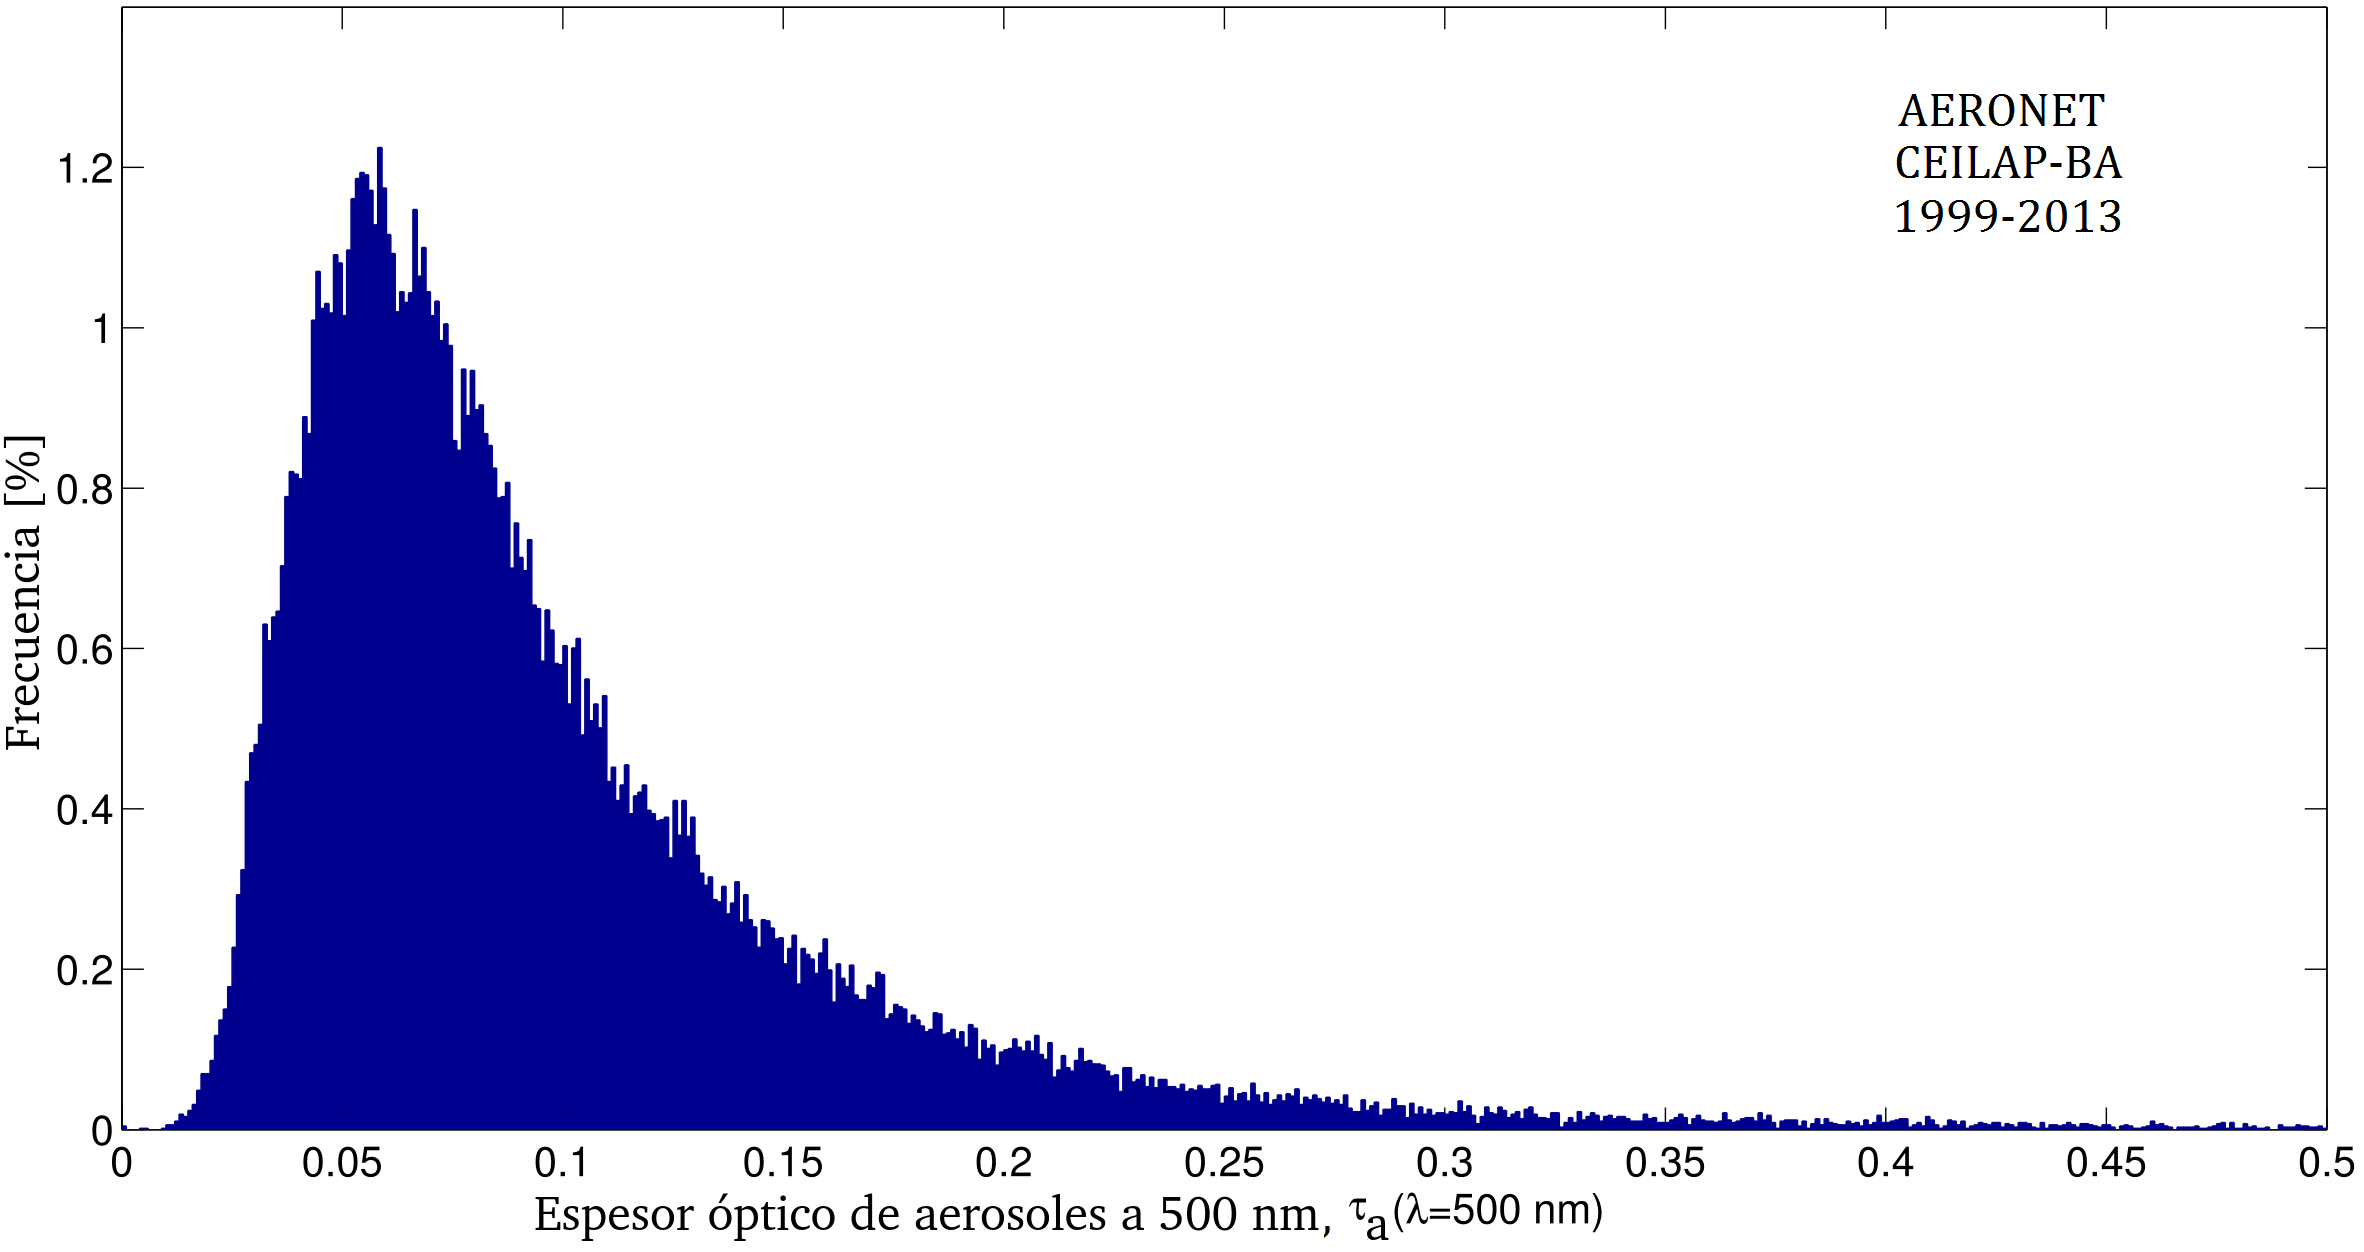
\includegraphics[width=3.0in]{pca/figures/TAU_AERONET.png}
\caption{Histogram of aerosol optical depth at 500 nm, as measured in CEILAP-BA (AERONET), period 1999-2013.}
\label{pca:tauaeronet}
\end{figure}

Las profundidades ópticas de aerosol a 500 nm, $\tau_{AER}(500)$, se determinaron a partir de las mediciones fotométricas realizadas en la estación CEILAP-BA [12], correspondientes a la red AERONET [13], en el período 1999-2013 (Figura 1). Estos valores se distribuyen log-normalmente en el rango de 0.00-0.50 con un valor de modo de 0.06. Los valores de reflectancia marina utilizados (denominados RdP 1, 2, 3 y 4, ver Fig. 2) corresponden a mediciones recopiladas durante dos campañas de campo en Punta Piedras, ubicadas en la zona de turbidez máxima del RdP, realizadas el 27 de febrero y el 30 de abril. , 2013 (estaciones PP01-07 / 02 y PP02-09 / 11 respectivamente). La reflectancia del agua (350-2500 nm) se midió usando un espectrómetro ASD Fieldspec FR. Los valores de turbidez medidos durante estas campañas aumentaron de RdP1 a RdP4, con valores que van desde 16 FNU (unidades nefelométricas de formacina) en RdP1 a> 1000 FNU (saturación del sensor) en RdP4 y se obtuvieron utilizando un turbidímetro portátil HACH 2100P ISO (ver Dogliotti et al. al. 2011 para ubicaciones y detalles [14]). Sobre estas reflectancias, se añadió el efecto de los casquetes blancos en las simulaciones, que se consideró dependiente de la velocidad del viento, como se describe en [15]-[17].

\begin{figure}
\centering
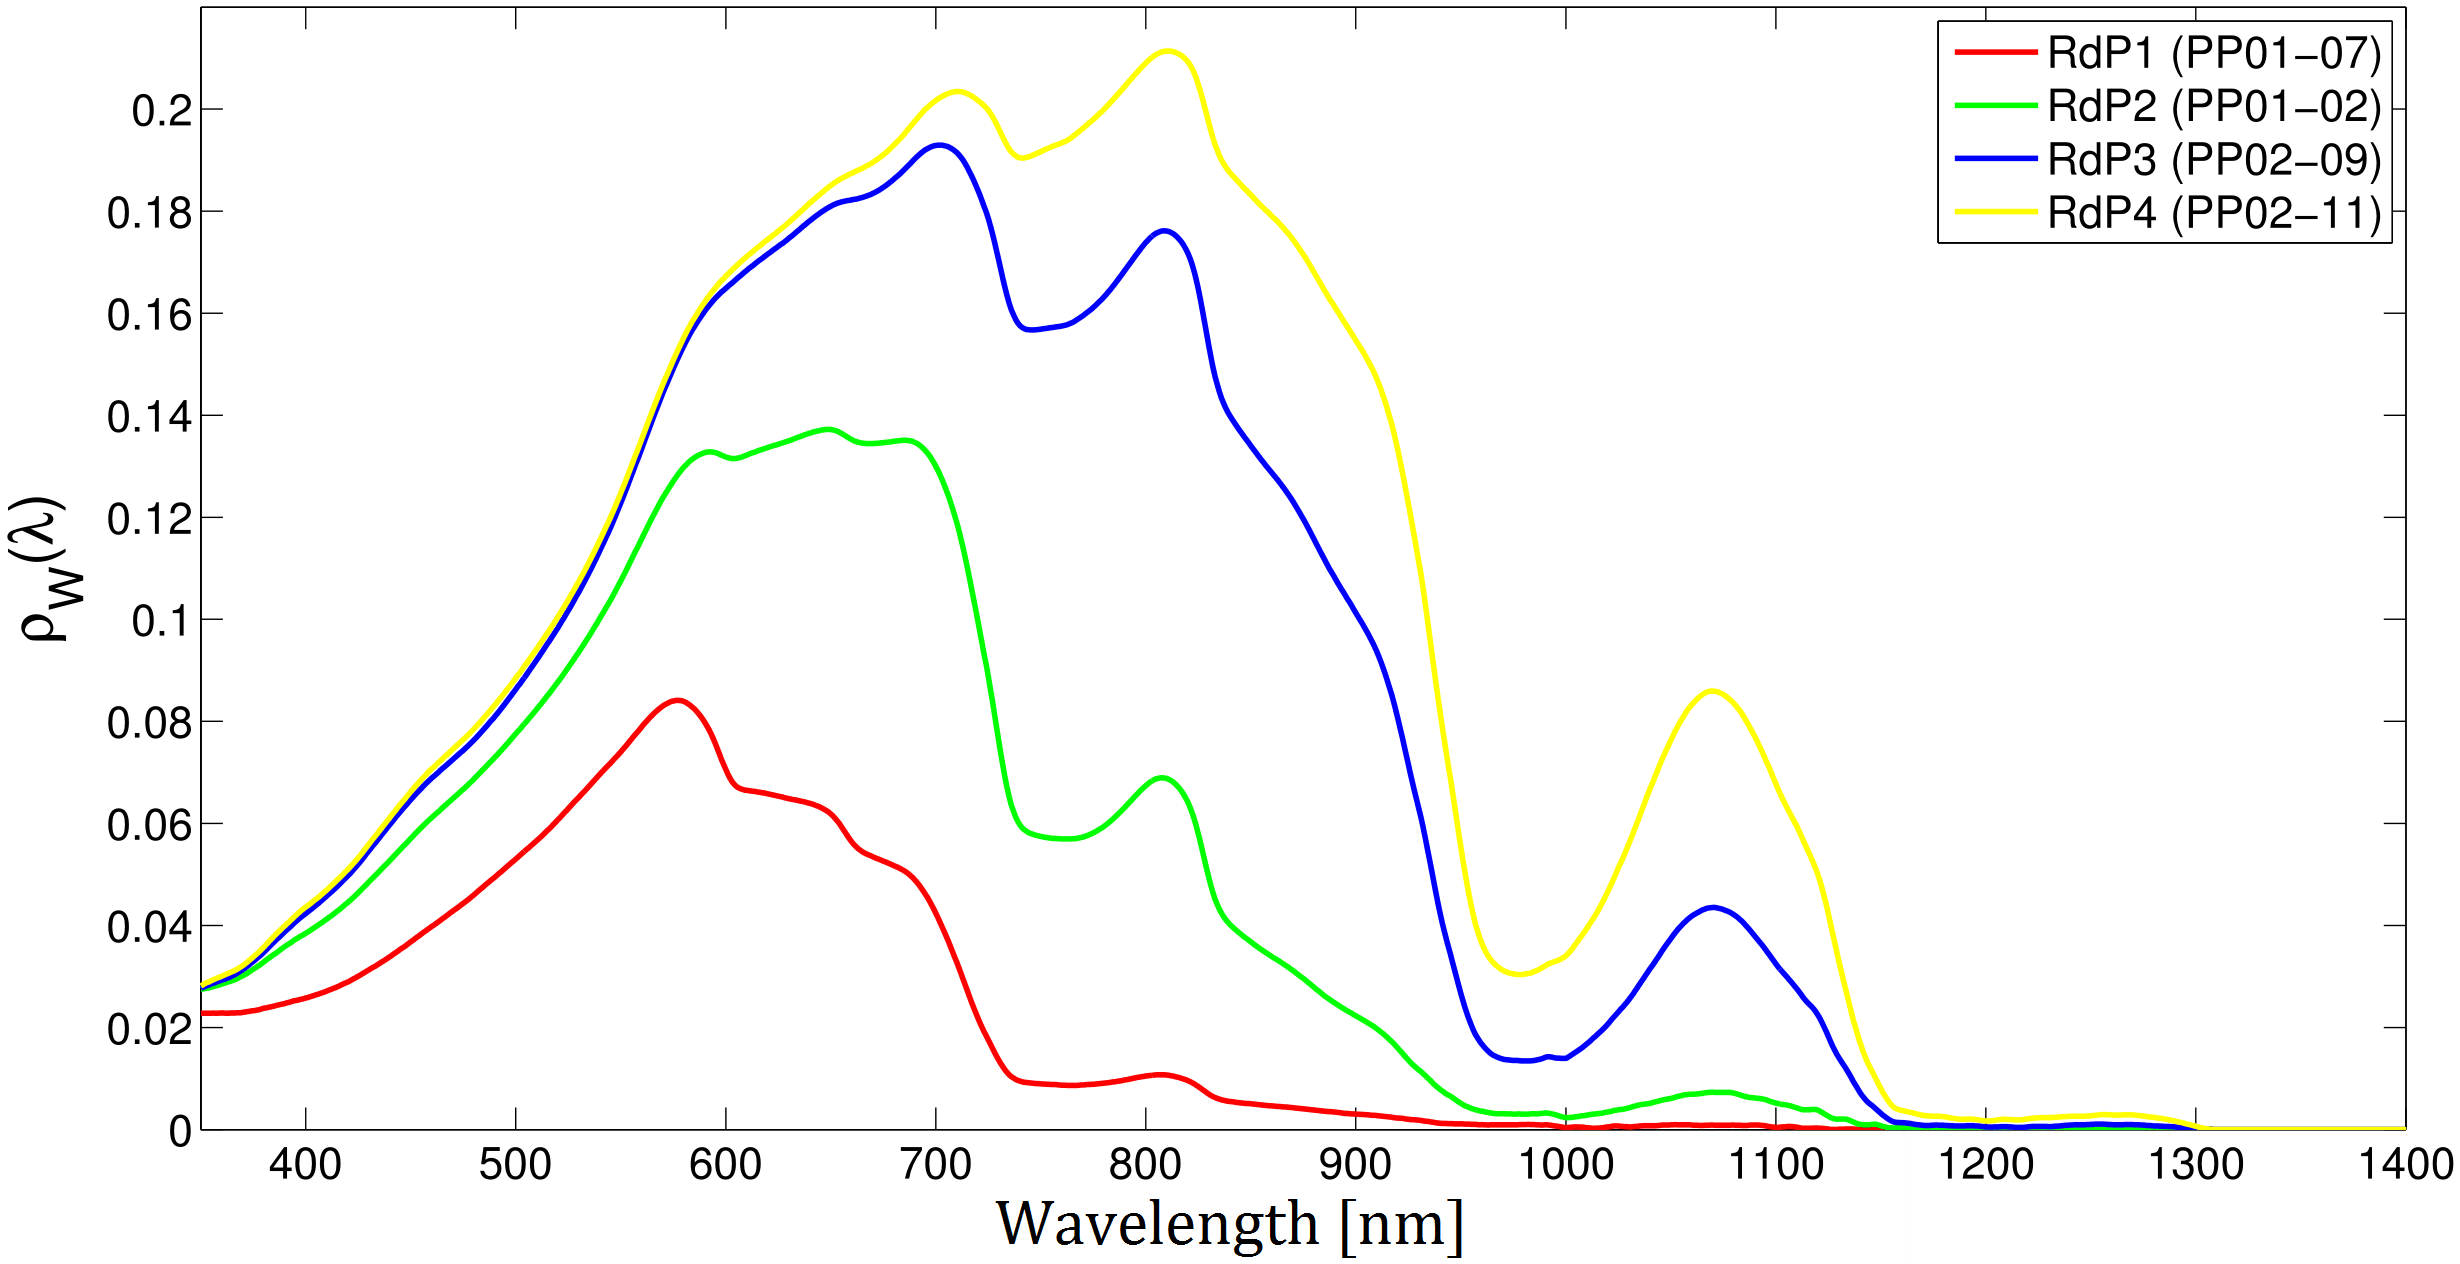
\includegraphics[width=3.0in]{pca/figures/RHOW_PTA_PIEDRAS.png}
\caption{Water reflectances (used as input to SOS code) obtained from field campaigns in Punta Piedras (Southern RdP) in the turbidity front region on February 27 and April 30, 2013.}
\label{pca:rhow_pta_piedras}
\end{figure}

El rango de velocidades del viento en la superficie (utilizado por SOS para calcular el término de superficie especular y la fracción de la superficie cubierta por espuma o \textit{whitecaps}) se seleccionó en función de los valores de viento medidos en la Estación Meteorológica Aeroparque para el período 1976-2014 (Fig. 3). Las velocidades de viento más probables corresponden al rango de 4-6 m/s, y los vientos superiores a 14 m/s se registraron en mucho menos del 1\% de las mediciones.

\begin{figure}
\centering
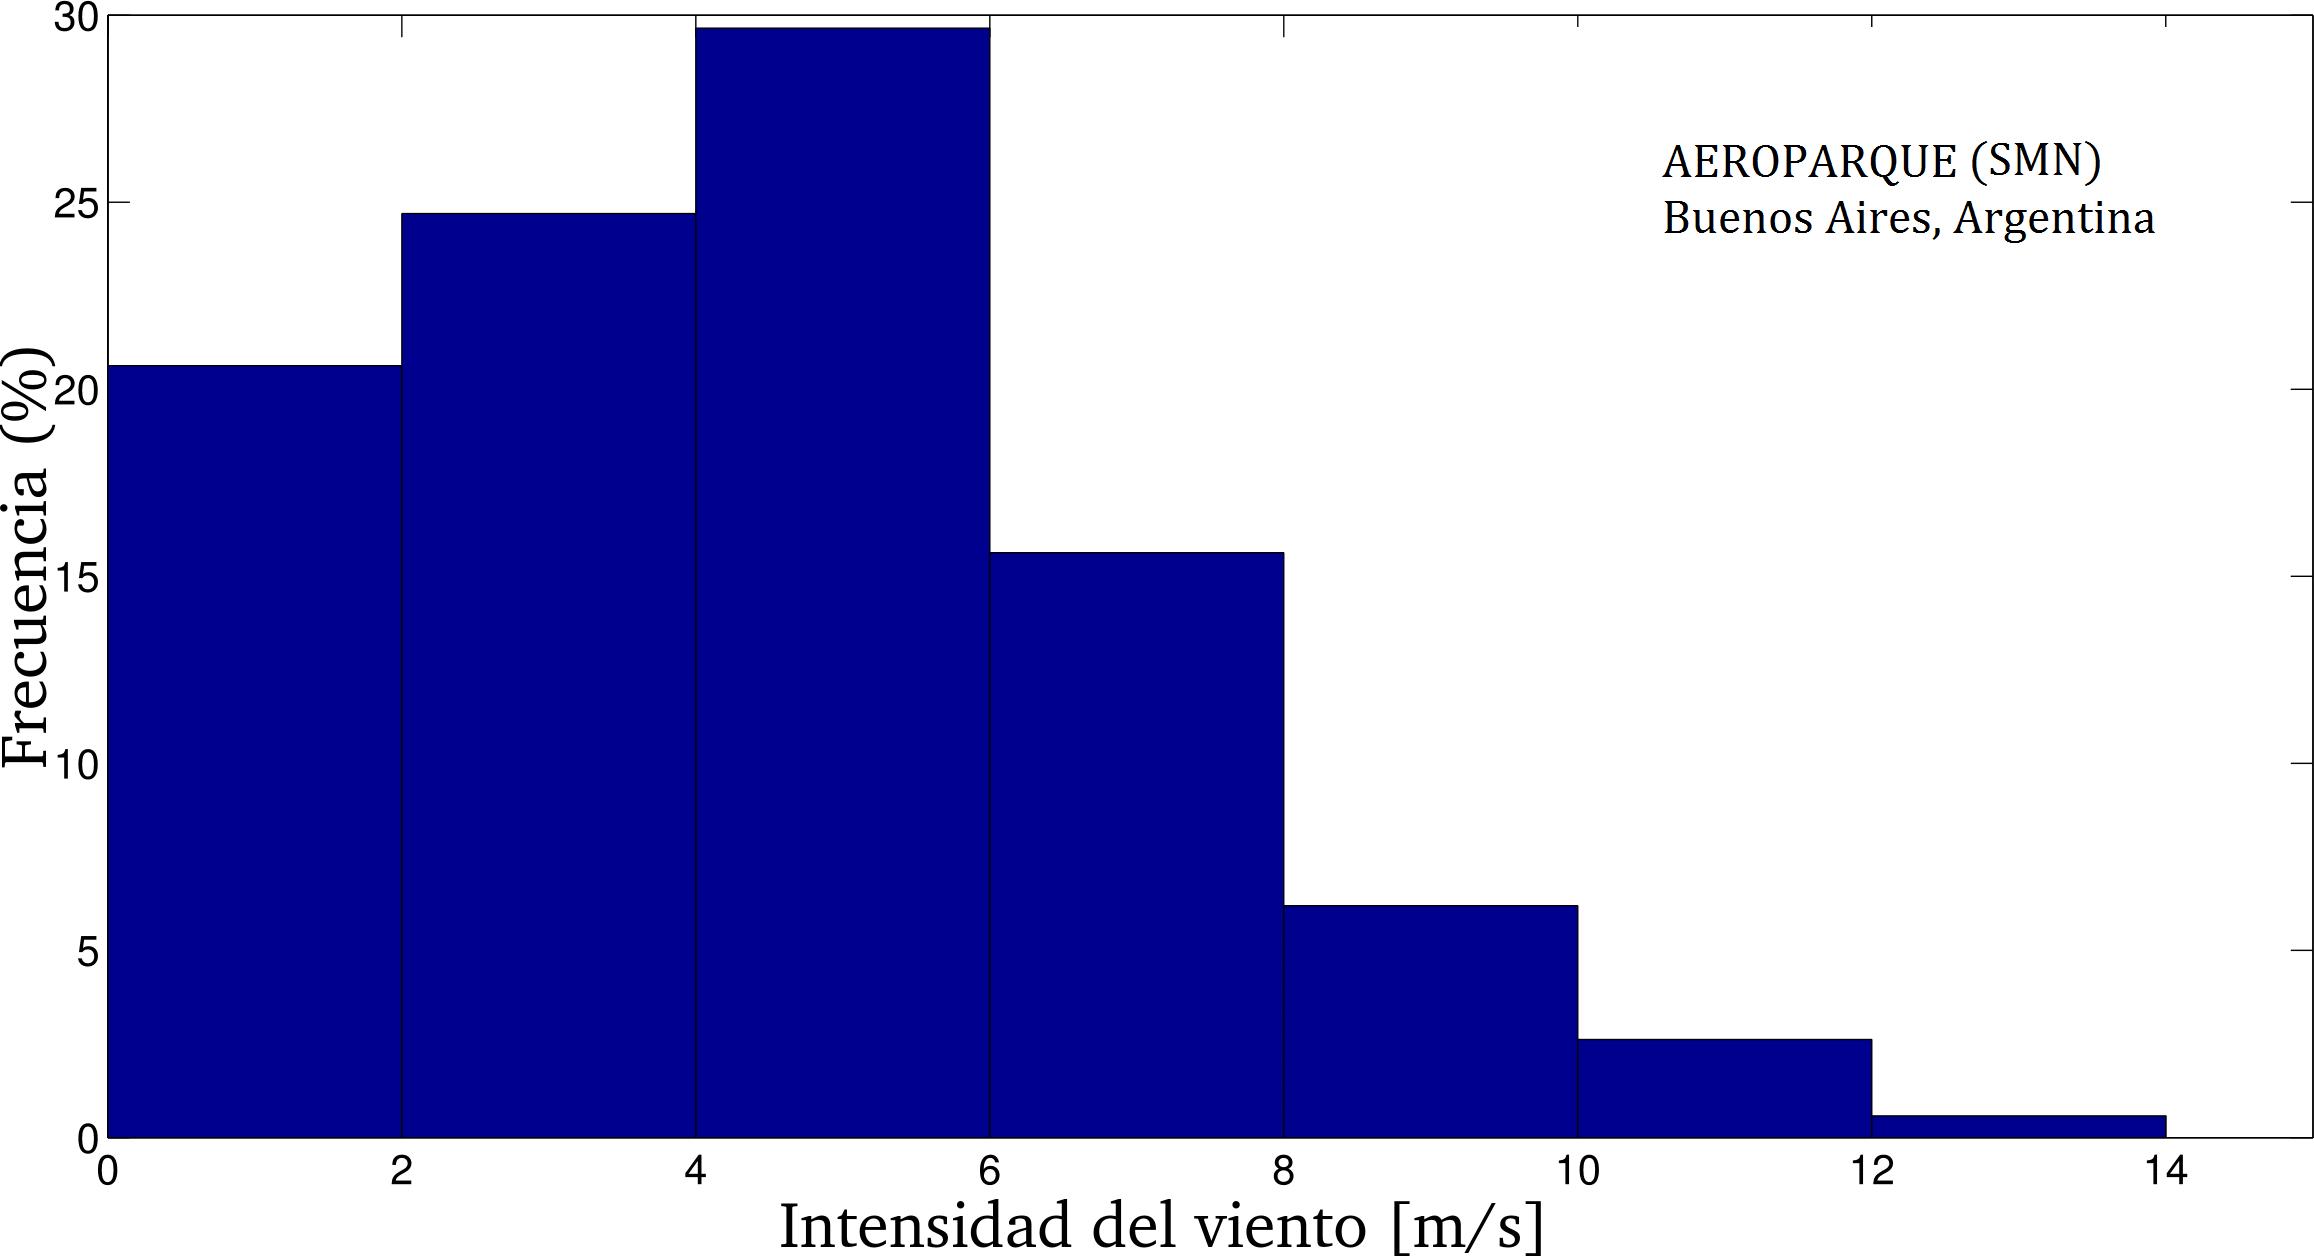
\includegraphics[width=3.0in]{pca/figures/VIENTO_AEROPARQUE.png}
\caption{Wind speed distribution of measurements taken at Aeroparque Meteorological Station, Buenos Aires, Argentina. Period 1976-2014.}
\label{pca:viento_aeroparque}
\end{figure}

Se calcularon los componentes I, Q y U de los parámetros de Stokes (es decir, se tomaron en cuenta los efectos de polarización, ver Lenoble et al. 2007 para más detalles [8]) para un máximo de 20 eventos de dispersión para cada fotón. El resto de las entradas requeridas por el SOS se fijaron a partir de los valores estándar encontrados en la literatura. Todos los valores utilizados se resumen en la Tabla III.

Se ejecutaron dos conjuntos separados de simulaciones. Se generó el primero introduciendo un océano negro para obtener la señal correspondiente a la atmósfera y la reflexión de la interfaz atmósfera-agua, definida como $\rho_{ATM}$. A partir de este conjunto, se calculó la descomposición de PCA, que produjo una base ortogonal de componentes principales, que corresponden a los vectores propios de la matriz de varianza-covarianza del conjunto, siendo el componente j-ésimo expresado como

\begin{equation}
e^{PCA}_{j}[\lambda,SWIR]    
\end{equation}

donde $j=1,...,N+1 $, siendo $N+1$ igual al número $N$ de bandas SWIR utilizadas para la corrección ($N=2$ o $3$, según el esquema) más la banda NIR en 865 nm.
El segundo conjunto corresponde a la señal simulada a TOA con océano no negro, es decir, incluye las reflectancias del agua que se muestran en la figura 2. Este conjunto de datos se utilizó para probar teóricamente el rendimiento de la corrección atmosférica.

Luego de i) asumir la condición de píxel negro en las bandas SWIR, ii) descartar regiones de valores elevados de brillo solar ($\rho_{SG}>0.050$); iii) desestimando el efecto de \textit{whitecaps} y la absorción gaseosa (despreciable en las bandas consideradas, dado que estas se hallan en ventanas atmosféricas), se obtiene la siguiente expresión para la reflectancia TOA:

\begin{equation}
\rho_{TOA}(865) \approx t(865)\rho_{w}(865) + \rho_{ATM}(865)
\\
\rho_{TOA}(SWIR) \approx \rho_{ATM}(SWIR)
\end{equation}

siendo $t(\lambda)$ la transmitancia atmosférica difusa y $\rho_{w}(\lambda)$ la reflectancia marina.
Usando las componentes principales de la señal $\rho_{ATM}$ (primer conjunto de simulaciones, ecuación (1)) y las reflectancias TOA en las bandas SWIR, $\rho_{TOA}(SWIR)$, las proyecciones a1 y a2 de las primeras dos componentes principales (en adelante consideraremos $N=2$ por brevedad) se calcularon invirtiendo el siguiente sistema lineal:

\begin{equation}
    \begin{pmatrix}
    \rho_{TOA}(SW1)\\ 
    \rho_{TOA}(SW2)
    \end{pmatrix}
    = 
    \begin{pmatrix}
    e_{1}^{PCA}(SW1) & e_{2}^{PCA}(SW1)\\ 
    e_{1}^{PCA}(SW2) & e_{2}^{PCA}(SW2)
    \end{pmatrix}
    \begin{pmatrix}a_{1}\\ 
    a_{2}
    \end{pmatrix}
\end{equation}

Luego, $\rho_{ATM}(865)$ se obtiene como combinación lineal de las proyecciones de más aporte a la varianza:

\begin{equation}
    \rho_{ATM}(865) \approx a_{1}e_{1}^{PCA}(865) + a_{2}e_{2}^{PCA}(865)
\end{equation}

y es sustraída de la señal, dejando el componente $t(865)\rho_{w}(865)$ (vea la ecuación (2)).
Finalmente, la señal restante se divide por la transmitancia difusa a 865 nm, $t(865)$, siguiendo la expresión sugerida en Tanre et al. 1979 [18]:

\begin{equation}
t(865) = exp\{-[0.52\tau_{RAY} + 0.16\tau_{AER}]/\mu\}
\end{equation}


donde los coeficientes 0.52 y 0.16 representan la fracción de retrodispersión respecto al total para moléculas y aerosoles, respectivamente; los espesores ópticos de Rayleigh y aerosoles a 865 nm se expresan respectivamente como $ \tau_{RAY}(865)$ y $\tau_{AER}(865)$, y $\mu$ representa el factor de masa de aire, $\mu = 1/cos(\theta_{S}) + 1/cos(\theta_{V})$, donde $\theta_{S}$ y $\theta_{V}$ son los ángulos cenitales solar y de observación. El valor de $\tau_{AER}(865)$ se fijó en la moda obtenida de la estación AERONET CEILAP-BA: $\tau_{AER}(865)=0.04$. La diferencia entre este valor y el real puede conducir a errores en el factor de transmitancia de 3-5\% en los peores casos.


Four different schemes were proposed with different MODIS (MD) and SABIA-Mar (SM) SWIR band combinations (shown between parentheses). They are:
PCA-2-SM (1240, 1640): uses 1240 nm band, which can have slightly non-zero marine signals in RdP (see Fig. 2).
PCA-2-MD (1640, 2130): Both bands used are effectively free from marine signal. 
PCA-3-SM (1044, 1240, 1640): Uses 1044 nm band, with moderate/high marine signals in RdP (see Fig. 2).
PCA-3-MD (1240, 1640, 2130): 1240 nm band was added to PCA-2-MD to enhance correlation with 865 nm.

A scheme summarizing the methodology is shown in Fig. 4.

\section{Resultados y discusión}
Some examples of TOA refleclectances retrieved by SOS using input parameters (indicated in Table III) are shown in Fig. 5. In the figure, the atmospheric scenario was set to 80\% Continental + 20\% Urban (Table II) for $\tau_{AER}(500)=0.5$ (green lines), while atmospheres free of aerosols correspond to $\tau_{AER}(500)=0$ (red lines), and scenarios corresponding to field measured reflectance spectra RdP1 and 4 (blue lines) were considered. The TOA signal seems consistent with what is expected, i.e., the shape and high signal associated to Rayleigh scattering is clearly observed in the blue region and the strong marine signal in the 500-1000 nm region; as well as becoming close to zero in the scenarios free of aerosols in the SWIR, while in the scenarios with aerosols still persists a strong flat signal in this spectral region.

\begin{figure}
\centering
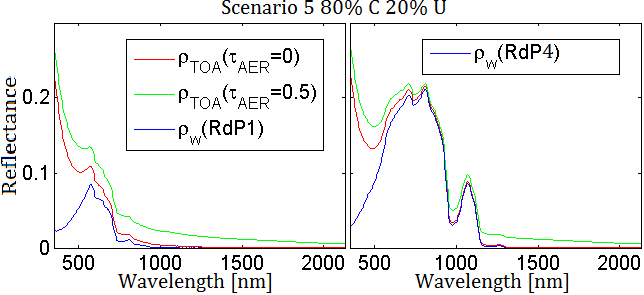
\includegraphics[width=3.0in]{pca/figures/RHO_TOA}
\caption{Simulated reflectances at TOA, corresponding to no aerosols and atmospheric scenario 5 with $\tau_{AER}(500)=0.5$ (red and green lines respectively) and field marine reflectances (blue lines), for RdP measurements 1 (left) and 4 (right)}
\label{pca:rho_toa}
\end{figure}

This behavior of the TOA signal as well as in the rest of the marine and atmospheric scenarios (not plotted here for brevity) brings confidence in the plausibility of the SOS simulations. Regarding the set simulated with $\rho_{w}=0$ (i.e. $\rho_{TOA}=\rho_{ATM}$), the scatter plots between the signal at the different bands is shown in Fig. 6.

\begin{figure}
\centering
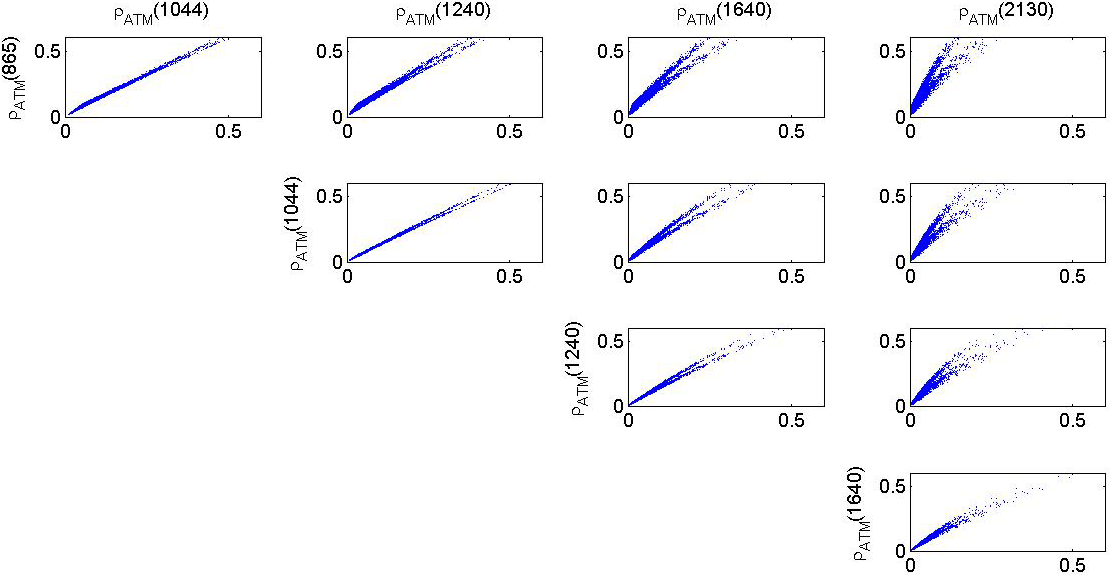
\includegraphics[width=3.0in]{pca/figures/RHO_ATM.png}
\caption{Scatter plots of the whole set of $\rho_{ATM}$ simulations for the NIR-SWIR bands considered (MODIS and SABIA-Mar band at 1044 nm)}
\label{pca:rho_atm}
\end{figure}

Estos gráficos muestran que existe una alta correlación entre la señal $\rho_{ATM}$ de las diferentes bandas SWIR; pero esta correlación tiende a disminuir a medida que aumenta la distancia espectral entre las bandas correspondientes. El esquema de PCA (ecuaciones (3) - (5)) se basa fuertemente en esta alta correlación, lo que significa que el uso de las bandas más distantes (es decir, las menos correlacionadas con 865 nm) puede traer más dispersión cuando se descartan los componentes principales con menos varianza asociada. Esto significa que existe una situación de compensación entre i) la validez de la suposición de píxel negro (completamente válida a 1640 y 2130 nm) y ii) la correlación entre $ \rho_{ATM}$ en la banda SWIR correspondiente y en 865 nm (peor para las bandas de 1640 y 2130 nm). 

The particularly separated plumes observed in the subplots corresponding to the highest spectral distances among bands (e.g. 865 vs 2130 nm, top-right corner, Fig. 6) are related to the presence of oceanic aerosols in the atmospheric scenarios proposed (particularly, Scenario 4, see Table II), which contain different absorption properties than the rest of the aerosol modes [11].
The results of the PCA atmospheric schemes for the four combinations of the MODIS/SABIA-Mar SWIR bands, described in detail in Section III, are shown in Fig. 7. For each scheme a linear regression was performed, shown with solid blue lines (slope, intercept and Pearson coefficient reported on each inset), while the 1:1 relation is indicated with a dashed black line. The PCA-3-SM (1044, 1240, 1640) scheme (third subplot, blue dots) presents highly underestimated values, mainly because it relies on the 1044 nm band, which presents a considerably high marine signal (see Fig. 2). For instance, this scheme is the one that better performs in the water scenario RdP 1, corresponding to the lowest $\rho_{w}(859)$ (Field) (vertical blue strip of the data in this subplot, see also Fig. 9). The rest of the PCA-derived reflectances from the other schemes present much higher scatter. This is linked to the fact that these schemes use bands further apart in the spectrum compared to PCA-3-SM, i.e., less correlated to 865 nm. For instance, the PCA-2-MD (1640, 2130) scheme (second subplot, green dots), which uses the two bands located farthest to 865 nm band presents the highest scatter.

\begin{figure}
\centering
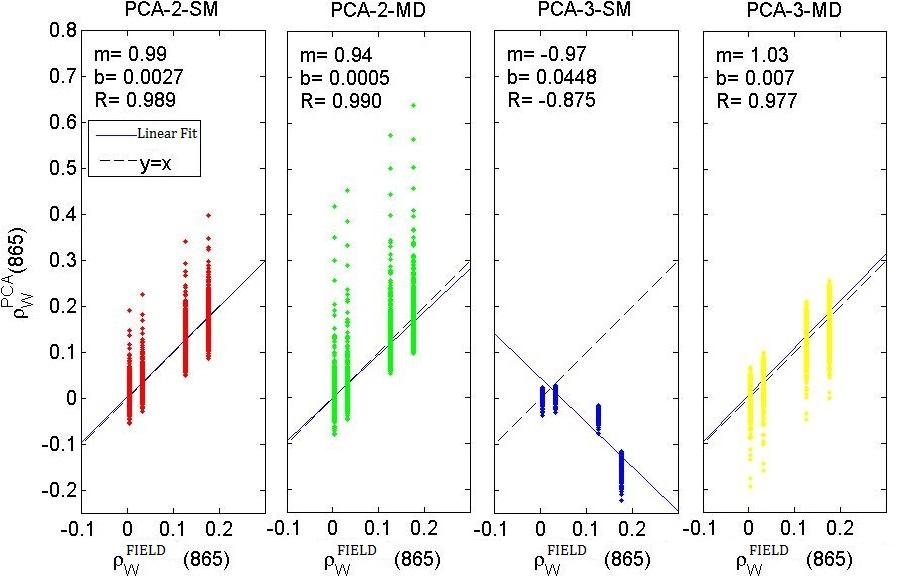
\includegraphics[width=3.0in]{pca/figures/PCA_GLOBAL}
\caption{Water reflectance $\rho_{w}(865)$ (FIELD) vs. $\rho_{w}(865)$ (PCA) for the four schemes proposed (PCA-2/3-SM/MD) and the four water scenarios considered, RdP 1-4 (four different values in x axis).}
\label{pca:pca_global}
\end{figure}

A series of subsets of the $\rho_{TOA}$ simulations were defined by setting reduced ranges for the input values reported in Table III to see if there existed a particular subset of the whole parametric set that resulted in the worse performances for the schemes (i.e. the parameter values associated to the most distant dots to the y=x line in Fig. 7). In particular, constraining the ranges of $\tau_{AER}(500)$ (aerosol optical thickness at 500 nm) and $\theta_{V}$ (viewing zenith angle) by the additional conditions:

\begin{equation}
\tau_{AER}(500) < 0.4\\
\theta_{V}<60\deg
\end{equation}

a new $\rho_{TOA}$ set is obtained and the results of the PCA performances are shown in Fig. 8. The conditions expressed in Eq. (6) exclude scenarios where: i) $\tau_{AER}(500)$ exceeds 0.4, i.e. very rare conditions based on in-situ measured values as shows Fig. 1, and ii) where the sensor is 30° or less above the horizon, i.e. corresponding to pixels located generally at the edge of the images that are usually discarded given the decreasing in the water reflectance that reaches TOA due to the larger atmospheric path length. The performance of the PCA algorithm over this reduced set is substantially improved over all schemes, except for PCA-3-SM (1044, 1240, 1640), that still presents high underestimation associated to non-zero water reflectance in 1044 nm band. 


\begin{figure}
\centering
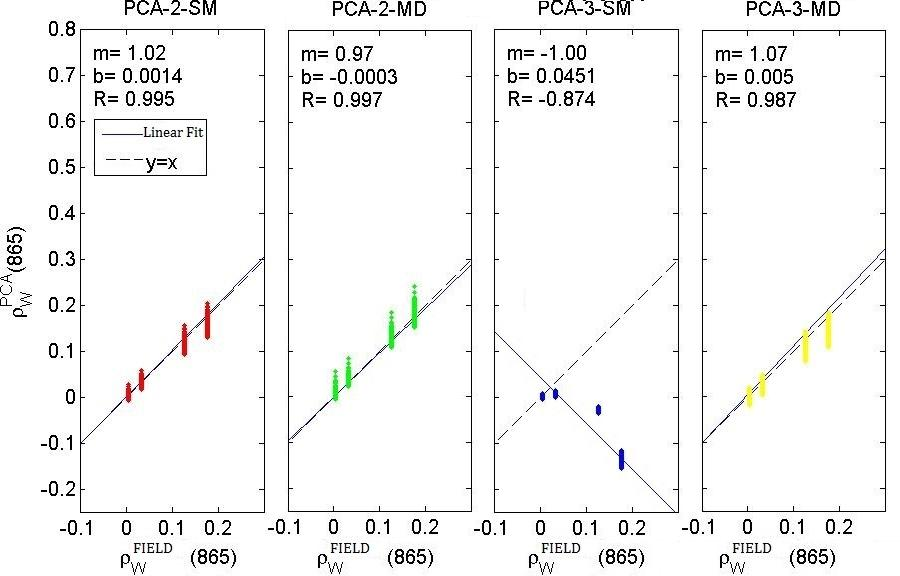
\includegraphics[width=3.0in]{pca/figures/PCA_REDUCIDO}
\caption{Same as Fig. 7 but for the reduced set as described in Eq. (6).}
\label{pca:pca_reducido}
\end{figure}

Finally, the absolute mean errors are shown in Fig. 9, for each of the schemes (PCA-2/3-SM/MD) and water scenarios (RdP 1-4), corresponding to the reduced $\rho_{TOA}$ set defined by Eq. (6). For the less turbid scenario (RdP1), with virtually no water signal in any of the tested SWIR bands, the schemes that show better performances are the ones that include the bands closet to 865 nm, i.e. the bands that exhibit highest correlation to 865 nm (in the $\rho_{ATM}$ signal, see Fig. 6). As the water scenarios exhibit higher water signals in the 1044 and 1240 nm bands, the schemes that use these bands tend to perform progressively worse, especially PCA-3-SM (1044, 1240, 1630, blue line), that correspond to the only scheme that includes the 1044 nm band. In the most turbid scenario (RdP4), with higher signal in the NIR-SWIR region, the scheme that performs better is PCA-2-MD (1640, 2130, green line): this can be attributed to the fact that this scheme is the only one that uses bands where the water signal is negligible.

\begin{figure}
\centering
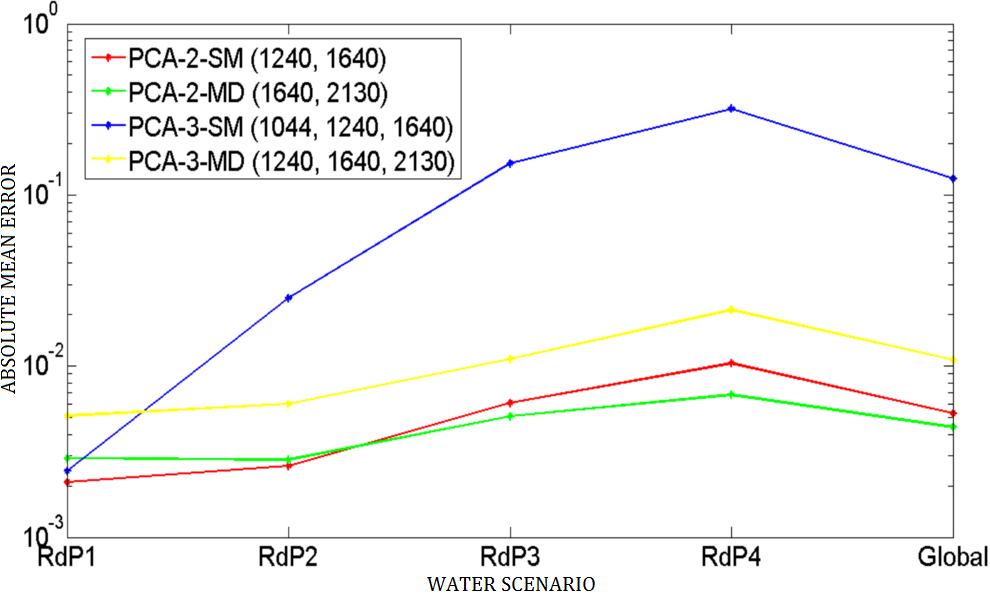
\includegraphics[width=3.0in]{pca/figures/PCA_mean_errors.png}
\caption{Mean absolute error for the different PCA schemes and field measured water reflectance, as well as the global performance.}
\label{pca:pca_mean_errors}
\end{figure}

\section{Conclusiones}

En el presente trabajo, se describe un algoritmo de corrección atmosférica diseñado para estimar la señal marina en la banda de 865 nm presente en los sensores MODIS y SABIA-Mar. Este algoritmo consiste en descomponer un conjunto de reflectancias simuladas de la componente atmosférica en componentes principales y estimar sus pesos correspondientes utilizando la reflectancia a tope de la atmósfera en las bandas SWIR (1000-3000 nm) en cada píxel. El algoritmo se probó teóricamente utilizando un conjunto de datos de reflectancias simuladas a TOA. Todas las simulaciones se obtuvieron utilizando el código de transferencia radiativa CNES-SOS, que se ejecutó utilizando parámetros de entrada restringidos utilizando condiciones atmosféricas medidas y datos de campo recopilados en la región del Río de la Plata (Argentina-Uruguay) y diferentes escenarios estándares de aerosoles. El RdP es uno de los ríos más turbios del mundo y, debido a sus altas concentraciones de partículas, estas aguas infringen la suposición de señal marina nula utilizada como punto de partida de los algoritmos de corrección atmosférica estándar en el NIR e incluso en las bandas SWIR de 1044 nm y 1240 nm.

Four different schemes were proposed which used different combinations of SWIR bands present in MODIS and SABIA-Mar sensors. Two conditions influenced the performance of each of the schemes: the presence of marine signal in the correcting (SWIR) bands and the spectral distance to the band of interest, i.e. 865 nm. Schemes using the nearest bands (1044, 1240 nm) had better performances for clear water scenarios while the ones that used black-ocean bands where the ocean is actually black (1640, 2130 nm) were the ones that performed better for the extremely turbid scenarios.